\documentclass{article}

\usepackage[margin=0.75in]{geometry}
\usepackage{amsmath,amssymb}
\usepackage{graphicx,float}
\usepackage{multirow,setspace}
\usepackage{natbib,enumerate}
\usepackage{caption}
\usepackage{subcaption}
\usepackage{termcal} 
\usepackage{xcolor}
\usepackage{enumitem}
\usepackage{gensymb}
\usepackage{booktabs}
\usepackage{listings}

\setlength{\marginparwidth}{2cm}

\renewcommand{\thesection}{\Alph{section}}
\newcommand{\HRule}{\rule{\linewidth}{0.5mm}}
\newcommand{\tab}{\hspace{0.5cm}}
\newcommand{\modref}[1]{(\ref{#1})}

\newcommand{\bbeta}{{\mbox{\boldmath$\beta$}}}
\newcommand{\bmu}{{\mbox{\boldmath$\mu$}}}
\newcommand{\balpha}{{\mbox{\boldmath$\alpha$}}}
\newcommand{\btheta}{{\mbox{\boldmath$\theta$}}}
\newcommand{\bpi}{{\mbox{\boldmath$\pi$}}}
\newcommand{\R}{\texttt{R}}
\newcommand{\Lik}{\mathcal{L}}

\begin{document}

%%% HEADER %%%
	\begin{center}
		\HRule \\[0.1cm]
		\vspace{0.1cm}
		{ \LARGE \bfseries MATH 2625: Biostatistical Methods\\[0.5cm] Homework 2, due Tuesday, February 11 } \\[0.1cm]
		\HRule \\[0.1cm]
	\end{center}
	
	Please submit a PDF or .doc version of your homework to Canvas by 3:30pm on the due date. Please type \emph{all} responses. You are encouraged to use \R\ for all calculations.
		
	\section*{Theory}
	\begin{enumerate}
		\item Suppose $m = {G \choose 2}$ tests are conducted for $G \in \mathbb{Z}^{+}$ and $> 2$. Let $X$ denote the RV that counts the number of rejected tests out of $m$. Under the null hypothesis that all $m$ null hypotheses are true, characterize the distribution of $X$ under each of the following rejection procedures:
		\begin{enumerate}
			\item Testing at the nominal $\alpha$ of 0.05.

			When a null hypothesis is true, this means that the probability of rejecting said test at the nominal level is $p = 0.05$. Suppose $Y$ was a random variable describing this binary outcome of either rejecting or failing to reject the null hypothesis (for each individual test). Then we can observe that
			
			$$Y \sim Bern(0.05).$$

			Since we defined $X$ as the random variable counting the number of rejected tests, this means that

			$$X \sim Bin(m, 0.05).$$

			\item Using the Bonferroni correction with nominal $\alpha$.
			
			When we apply a Bonferroni correction to the set of multiple hypothesis tests (with all null hypotheses still being true), then we observe that the random variable $X$ which counts the number of rejected tests takes on a binomial distribution similar to that described in part (a):

			$$X \sim Bin(m, \frac{0.05}{m}).$$

			\item Under the \v{S}id\'ak correction with nominal $\alpha$.
			
			The \v{S}id\'ak correction results in $X$ being binomial similar to the results demonstrated in (a) and (b):

			$$X \sim Bin(m, 1 - (0.95)^{1/m}).$$
			
		\end{enumerate}
		For each, justify your choice and state any necessary assumptions.
		

		\newpage
		\item Show Pearson's correlation coefficient, $r$, is a function of the OLS estimate, $\hat{\beta}_1$, i.e. show result on slide 146
		\begin{align*}
			r &= \frac{s_x}{s_y}\hat{\beta}_1,
		\end{align*}
		where $s_x$ and $s_y$ are the sample standard deviations of $x$ and $y$, respectively.

		Pearson correlation coefficent is defined as

		$$r = \frac{Cov(X, Y)}{\sigma_X \sigma_Y}.$$

		The simple linear regression formula is defined as

		$$Y = \beta_0 + \beta_1X + \epsilon,$$

		where $\epsilon \sim N(0, \sigma_\epsilon) $. When we substitute in estimators, we get

		$$Y = \hat\beta_0 + \hat\beta_1X + \epsilon,$$
		
		If we take the variance of both sides of this equation, then it becomes

		$$Var(Y) = Var(\hat\beta_0 + \hat\beta_1X + \epsilon).$$

		Since $\hat\beta_0$ is a constant, we know that $Var(\hat\beta_0) = 0$. We can rewrite this as

		$$Var(Y) = \hat\beta_1^2Var(X) + \sigma_\epsilon^2.$$

		When we take the square root of both sides, we get

		$$\sigma_Y = \sqrt{\hat\beta_1^2Var(X) + \sigma_\epsilon^2} $$

		When we plug this into the top equation, we get

		$$r = \frac{Cov(X, Y)}{\sigma_X \sqrt{\hat\beta_1^2Var(X) + \sigma_\epsilon^2}}.$$

		This shows that $\hat\beta_1$ is related to $r$.

		




	\end{enumerate}



	\newpage
	\section*{Case Study}
	For each of the following case studies, create a structured abstract no longer than 4 pages in length (including figures, tables, and references). The Background sections are provided for each and should be included in your write-up. You must write the Methods, Results, and Conclusion sections. Code should be included in an appendix as well.

	\begin{enumerate}
		\item In this case study, you will examine data on workers in the cadmium industry, focusing on a possible relationship between the level of exposure to cadmium and an indicator of lung health. The dataset is in the \texttt{ISwR} library and named \texttt{vitcap2}. It contains the variables \texttt{group} indicating cadmium exposure status (1 for exposed $>10$ years, 2 for exposure $<10$ years, and 3 for not exposed), each workers \texttt{age} in years, and each workers \texttt{vital.capacity}, measured in liters.
		
		\item The second case study considers a study of the lung functioning of patients with cystic fibrosis and how it relates to body mass as well as age. The data is alongside this assignment in the file \texttt{cf.txt} and contains the primary outcome of interest \texttt{fev1} (the forced expiratory volume in one second). The primary predictors of interest are \texttt{bmp} (body mass as a percent of normal binned to \texttt{very low}, \texttt{low}, and \texttt{near normal}) and \texttt{weight} (in \texttt{kg}). A possible confounder of interest, \text{age} in years, is included as well.
	\end{enumerate}

		\newpage
	\subsection*{Background}
				
		Vital capacity, a measure of lung volume defined as the maximum amount of air a person can expel from their lungs after taking a maximum inhalation, can be used to help diagnose underlying lung disease or dysfunction. If vital capacity is lower than expected, further testing for possible disease or other complications is warranted. Exposure to cadmium, even at low doses, may have impacts on kidney and bone health and at high levels may damage the lungs. Cadmium production increased considerably over the course of the 20th Century and is used across a number of different industries. To assess the potential impact exposure to cadmium might have, we examined the vital capacity in workers from industries that use cadmium in various production processes. Workers were randomly selected from nine different factories: eight PVC factories using cadmium stabilizers in the compounding of PVC and one cadmium-nickel battery factory. We classified the workers as having long term exposure ($>10$ years exposure to cadmium), short to medium term exposure ($<10$ years exposure), and no exposure. Our primary goal is to see if exposure to cadmium impacts the lung functioning of the workers in the industry. It is well known, however, that vital capacity also depends on a number of additional factors, including a person's age. Older workers may also be more likely to have longer periods of exposure, thus we also examine workers' age as a possible confounder.

	\subsection*{Methods}
		We tested the vital capacity (VC) of workers who were identified as either having long-term exposure (exceeding 10 years) or short term exposure (less than 10 years). We also randomly measured vitals from workers who had no exposure to form a control group. 12 workers with long-term exposure, 28 with short-term exposure, and 44 with no exposure were selected for the study.

		Analysis of the differences between vital levels was done nonparametrically using a Kruskal-Wallis Test at the nominal level. We also planned to conduct any necessary post-hoc tests using a Mann-Whitney U Test, with a Bonferroni correction to control for multiple tests.

		As a secondary analysis, we checked the influence of age as a confounding variable using Spearman’s rank coefficient. We checked for correlation between age and VC of all workers, and then separately in their respective groups (long-term exposure, short-term exposure, and the control group). A Bonferroni correction was applied to these four Spearman correlation tests, resulting in a corrected critical threshold of $\alpha^* = 0.0125$.
		
	\subsection*{Results}

		There was a greater variation in the vital capacities of workers who experienced long-term cadmium exposure. Additionally, one worker who faced short-term exposure had an unusually low VC. This outlier is shown in figure 2, along with the distributions of the boxplots of all the study cohorts. We did not find evidence to suggest that exposure to cadmium made a difference in the vital capacity of workers $(p = 0.2477, H = 2.790, df = 2)$.

		\begin{table}[h!]
			\centering
			\footnotesize
			\caption{\textbf{Summary of Vital Capacity of Workers in Every Group}}
			\begin{tabular}{lcccc}
				\toprule
				\textbf{} & \textbf{All Workers} & \textbf{Long-term Exposure} & \textbf{Short-term Exposure} & \textbf{Control} \\
				\midrule
				\textbf{Number of Workers} & 84 & 12 & 28 & 44 \\
				\textbf{Mean Age} \textit{(Years)} & 40.55 & 49.75 & 37.79 & 39.80 \\
				\textbf{Mean VC} \textit{(Liters)} & 4.392 $\pm$ 0.164 & 3.949 $\pm$ 0.656 & 4.472 $\pm$ 0.682 & 4.462 $\pm$ 0.692 \\
				\textbf{VC St. Dev.} \textit{(Liters)} & 0.757 & 1.033 & 0.682 & 0.692 \\
				\textbf{Median VC} \textit{(Liters)} & 4.530 & 3.865 & 4.615 & 4.530 \\
				\textbf{MAD} \textit{(Liters)} & 0.756 & 1.460 & 0.667 & 0.689 \\
				\bottomrule
			\end{tabular}
		\end{table}

		\newpage

		\begin{figure}[h!]
			\centering
			\tiny
			\begin{minipage}{0.48\textwidth}
			  \centering
			  \tiny
			  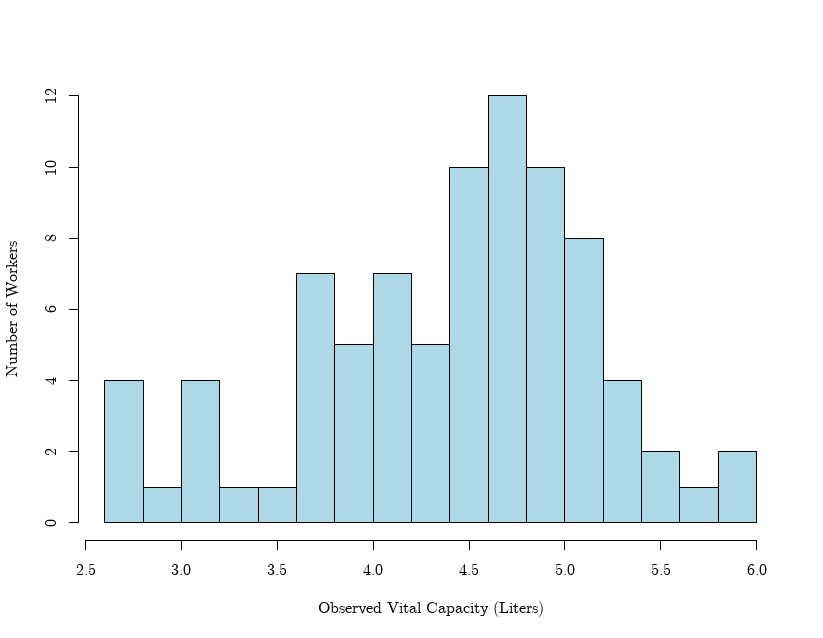
\includegraphics[width=\textwidth]{graphs/HistAllWorkers~VitalCap.png}
			  \caption{Histogram of Workers' Vital Capacity}
			  \label{fig:histogram}
			\end{minipage}\hfill
			\begin{minipage}{0.48\textwidth}
			  \centering
			  \tiny
			  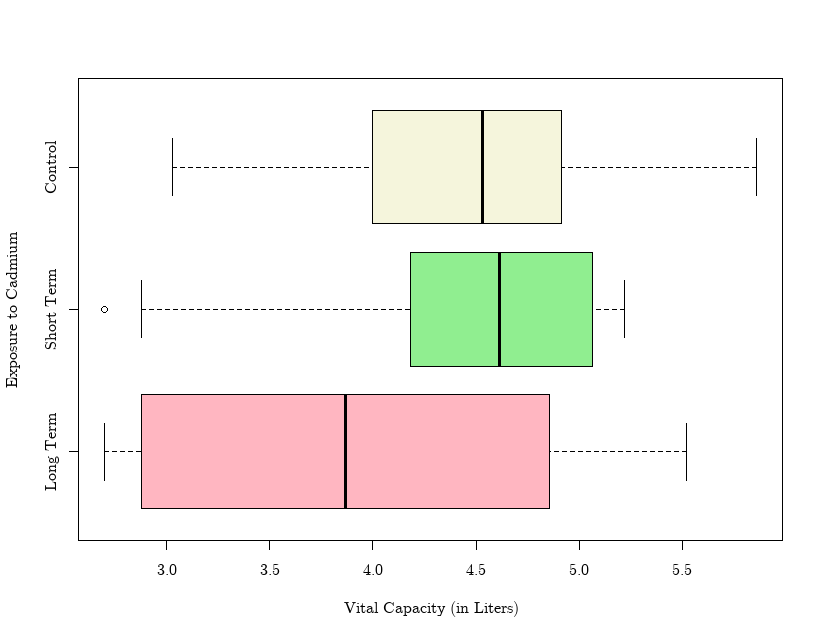
\includegraphics[width=\textwidth]{graphs/BoxPlot_Workers~VitalCap.png}
			  \caption{Boxplots of Vital Capacities Across Cohorts}
			  \label{fig:boxplots}
			\end{minipage}
		\end{figure}



		We found evidence to suggest that age is a confounding variable for determining vital capacity in this study. Worker age and vital capacity appear to be negatively correlated $(p < 0.001, \rho = -0.544)$. Figures 3 and 4 visualize this association, which also held true in all three cohorts of the study. Table 2 provides a summary of the negative correlation found between all exposure levels. Overall, age had a strong impact on the workers’ vital capacity regardless of exposure to cadmium.

		\begin{figure}[h!]
			\centering
			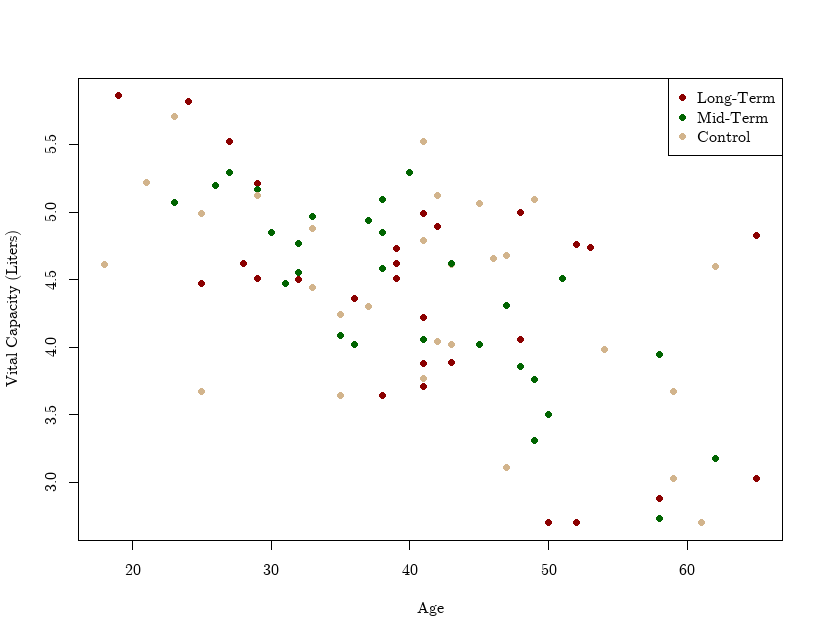
\includegraphics[width=0.6\textwidth]{graphs/ScatterAll.png}
			\caption{Worker Age and Vital Capacity Appear to be Negatively Correlated}
			\label{fig:histogram}
		\end{figure}

		\begin{table}[h!]
			\centering
			\footnotesize
			\caption{\textbf{Correlation Found Between Age and Vital Capacity Across all Exposure Levels}}
			\begin{tabular}{lccc}
				\toprule
				\textbf{Group} & \textbf{Spearman’s $\rho$} & \textbf{p-value} & \textbf{Significant at $\alpha^* = 0.0125$ }  \\
				\midrule
				All Workers & $-0.544$ & $<0.001$ & Yes \\
				Long-Term Exposure & $-0.747$ & 0.005 & Yes \\
				Short-Term Exposure & $-0.557$ & 0.002 & Yes \\
				Control & $-0.494$ & $<0.001$ & Yes \\
				\bottomrule
			\end{tabular}
		\end{table}

		\begin{figure}[h!]
			\centering
			\begin{subfigure}[b]{0.3\textwidth}
				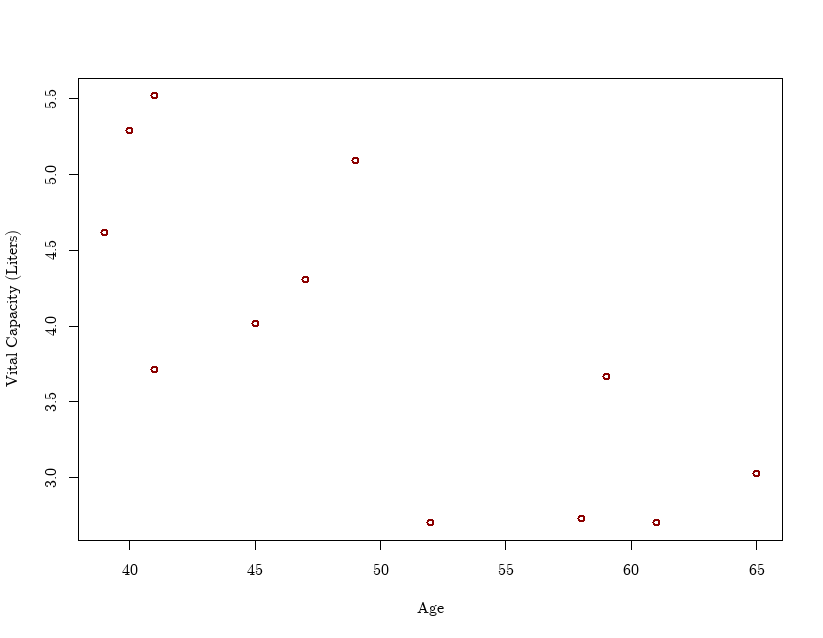
\includegraphics[width=\textwidth]{graphs/ScatterLongExp.png}
				\caption{Long-Term Exposure}
				\label{fig:img1}
			\end{subfigure}
			\hspace{0.05\textwidth} % Adds space between the images
			\begin{subfigure}[b]{0.3\textwidth}
				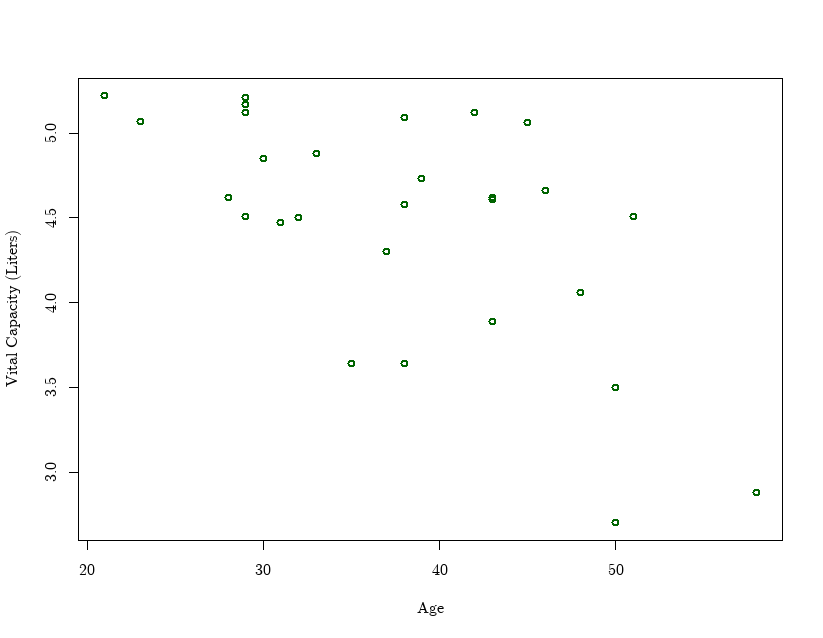
\includegraphics[width=\textwidth]{graphs/ScatterShortExp.png}
				\caption{Short-Term Exposure}
				\label{fig:img2}
			\end{subfigure}
			\hspace{0.05\textwidth}
			\begin{subfigure}[b]{0.3\textwidth}
				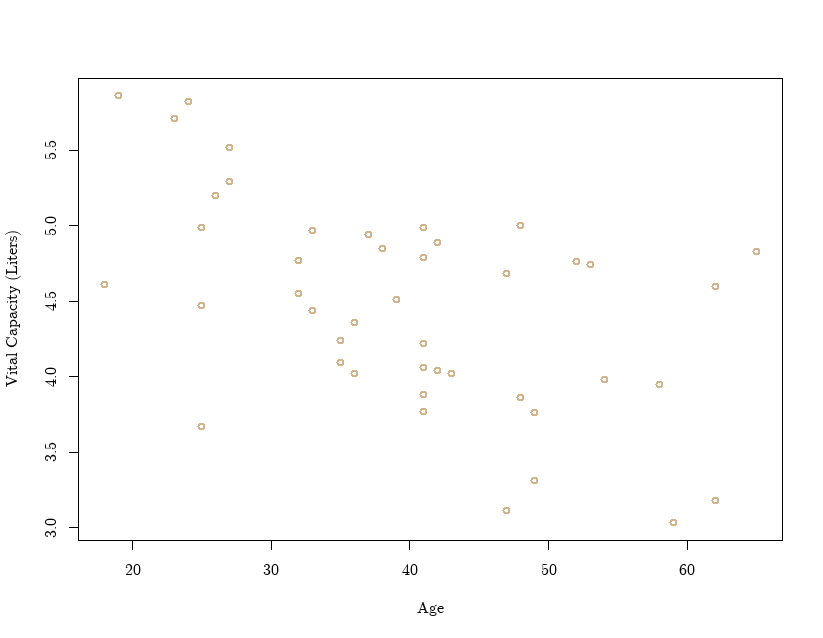
\includegraphics[width=\textwidth]{graphs/ScatterControl.png}
				\caption{Control Group}
				\label{fig:img3}
			\end{subfigure}
			\caption{Correlation between Age \& Vital Capacity Found Among All Subgroups of Study}
			\label{fig:three_images}
		\end{figure}

		\newpage

		\subsection*{Discussion}
		Although no difference in vital capacity was observed as a result of the different exposure lengths to cadmium, we observed substantial impacts from a worker’s age on their resulting vital capacity. This lack of statistically significant difference is corroborated by related findings in the literature. Though Yang and colleagues (2019) also did not find a significant difference in forced vital capacity (in short, a related but more effortful measure of vital capacity) per 1~\(\mu\)g/L blood serum cadmium in their multivariable regression models, they did find significant negative differences in other lung function metrics, patient-predicted FEV\(_1\) and FEV\(_1\)/FVC, with each additional \(\mu\)g/L cadmium. Wang and colleagues (2024) support this result, finding in their meta-analysis that per 1~\(\mu\)g/L cadmium exposure, FEV\(_1\)/FVC level decreased by 47.54\%, which was a statistically significant result. These findings may suggest that in order to capture the full picture of cadmium exposure and lung function, future research should explore including additional metrics like FEV\(_1\) or FEV\(_1\)/FVC alongside vital capacity.

		In terms of age and vital capacity, it is well documented that vital capacity declines with age over time (Cid-Juárez et. al., 2019). It is worth noting that the mean age of workers who faced long-term exposure was higher than both workers who only faced short-term exposure, workers with no exposure, and the overall group in general. This was one of the major limitations of the study and may have been due to the small number of workers who had long-term exposure. While it makes sense that workers who faced exposure for a longer period of time, a follow-up study should seek to address this by also finding older workers who faced short-term exposure and no exposure. It should also seek to sample a larger number of workers overall, as well as workers from a larger number of factories. This would help to address the issues related to internal and external validity that the study faces. Other factors found to influence vital capacity include gender, athleticism, and other pre-existing medical conditions that vary from person to person (Lemon \& Moersch, 1924; Abboud et. al., 2024), so future research should monitor these variables as well for possible confounding.

		\newpage
		\subsection*{Appendix}

		\begin{itemize}
			\item Abboud, H. J., Hussein, H. K., \& Fadhil, S. A. (2024). The effect of increasing the intensity of specialized endurance training on runners' ability in the advanced 1500-meter run in terms of vital capacity indicators (VC) and heart rate (SV). \textit{TechHub Journal}, 7, 19–27.

			\item Cid-Juárez, S., Thirión-Romero, I., Torre-Bouscoulet, L., Gochicoa-Rangel, L., Martínez-Briseño, D., Hernández-Paniagua, I. Y., Delgadillo-Ruiz, O., Guerrero-Zúñiga, S., Del Río-Hidalgo, R., Cortés-Medina, D., Bapo-López, P. E., León-Gómez, P., Bautista-Bernal, A., \& Pérez-Padilla, R. (2019). Inspiratory capacity and vital capacity of healthy subjects 9–81 years of age at moderate-high altitude. \textit{Respiratory Care}, 64(2), 153–160. 
			https://doi.org/10.4187/respcare.06284

			\item Lemon, W. S., \& Moersch, H. J. (1924). Factors influencing vital capacity. \textit{Archives of Internal Medicine}, 33(1), 136–144. 
			https://doi.org/10.1001/archinte.1924.00110250139014 

			\item Wang, Y., Wang, D., Hao, H., Cui, J., Huang, L., \& Liang, Q. (2024). The association between cadmium exposure and the risk of chronic obstructive pulmonary disease: A systematic review and meta-analysis. \textit{Journal of Hazardous Materials}, 469(133828). 
			https://doi.org/10.1016/j.jhazmat.2024.133828 

			\item Yang, G., Sun, T., Han, Y-Y., Rosser, F., Forno, E., Chen, W., \& Celadon, J. C. (2019). Serum cadmium and lead, current wheeze, and lung function in a nationwide study of adults in the United States. \textit{Journal of Allergy and Clinical Immunology: In Practice}, 7(8), 2653–2660. 
			https://doi.org/10.1016/j.jaip.2019.05.029 
		\end{itemize}

		\subsection*{R Code}
		\begin{lstlisting}[language=R, basicstyle=\footnotesize\ttfamily, breaklines=true]
			# Install necessary packages
			# install.packages('DescTools')
			# install.packages('Rfit')
			# Disclaimer: I used chatGPT to be able to display this in latex, hope that's okay
			library(ISwR) # data source
			
			# Formatting for LaTeX output
			library(showtext)
			library(DescTools)
			library(Rfit)
			font_add(family = 'ComputerModern', regular = 'cmunrm.ttf') # for consistent formatting in LaTeX
			showtext_auto()
			par(family = 'ComputerModern')
			
			# Load dataset
			data('vitcap2')
			
			# Subset data by exposure level
			noExposure = subset(vitcap2, group == '3')
			midExposure = subset(vitcap2, group == '2')
			longExposure = subset(vitcap2, group == '1')
			exposures = list(vitcap2 = vitcap2, 
							longExposure = longExposure,
							midExposure = midExposure, 
							noExposure = noExposure)
			
			# Loop through each group and compute summary statistics
			for (group_name in names(exposures)) {
			  group_data = exposures[[group_name]]
			  
			  vital_sd <- sd(group_data$vital.capacity)
			  n <- length(group_data$vital.capacity)
			  
			  margin = qt(0.975, df = n - 1) * (vital_sd / sqrt(n))  # margin for 95% CI
			  
			  # Print results
			  print(paste('Group:', group_name, '( N =', n, ')'))
			  print(paste('  Mean Age:', round(mean(group_data$age), 3))) 
			  print(paste('  Mean Vital Capacity:', round(mean(group_data$vital.capacity), 3),
						  '| SD:', round(vital_sd, 3)))
			  print(paste('  95% CI MoE:', round(margin, 3)))
			  print(paste('  Median VC:', median(group_data$vital.capacity)))
			  print(paste('  MAD:', mad(group_data$vital.capacity)))
			  print('')
			}
			
			# Histograms and boxplots
			hist(vitcap2$vital.capacity, col = 'lightblue', 
				 breaks = 12, ylab = 'Number of Workers',
				 xlab = 'Observed Vital Capacity (Liters)',
				 main = '')
			
			boxplot(vital.capacity ~ group, data = vitcap2, 
					main = '',
					xlab = 'Vital Capacity (in Liters)', 
					ylab = 'Exposure to Cadmium', 
					col = c('lightpink', 'lightgreen', 'beige'), horizontal = T,
					names = c('Long Term', 'Short Term', 'Control'))
			
			kruskal.test(vital.capacity ~ group, data = vitcap2)
			
			# Scatter plots and correlation
			plot(vital.capacity ~ age, data = vitcap2, 
				 col = c("darkred", "darkgreen", "tan"),
				 pch = 16,
				 xlab = 'Age', ylab = 'Vital Capacity (Liters)', 
				 main = '')
			
			legend("topright", legend = c("Long-Term", "Mid-Term", "Control"),
				   col = c("darkred", "darkgreen", "tan"), pch = 16)
			
			# Individual scatter plots
			plot(vital.capacity ~ age, data = longExposure, col = 'darkred',
				 xlab = 'Age', ylab = 'Vital Capacity (Liters)', lwd = 2)
			
			plot(vital.capacity ~ age, data = midExposure, col = 'darkgreen',
				 xlab = 'Age', ylab = 'Vital Capacity (Liters)', lwd = 2)
			
			plot(vital.capacity ~ age, data = noExposure, col = 'tan',
				 xlab = 'Age', ylab = 'Vital Capacity (Liters)', lwd = 2)
			
			# Spearman correlations
			with(vitcap2, cor.test(age, vital.capacity, method = 'spearman' ))
			with(longExposure, cor.test(age, vital.capacity, method = 'spearman' ))
			with(midExposure, cor.test(age, vital.capacity, method = 'spearman' ))
			with(noExposure, cor.test(age, vital.capacity, method = 'spearman' ))
			\end{lstlisting}


		\newpage
		\subsection*{Background}
		
		Cystic fibrosis is a genetic disorder that affects the lungs, among other major organs. A mutation in the cystic fibrosis transmembrane conductance regulator (CFTR) gene is the cause, resulting in the dysfunction of the CFTR protein which facilitates the transportation of chloride to the cell surface. Without the additional chloride, mucus lining the cells of vital organs becomes thick and viscous, clogging airways and resulting in difficulty breathing. Additional complications in increased risk of bacterial infection and respiratory failure. Poor growth or weight gain is a common complication as well, and often an early indicator of cystic fibrosis. To assess the relationship between growth and weight and lung functioning in patients with cystic fibrosis, we recruited 25 patients between the ages of 7 and 23 years old. Our primary outcome of interest is the forced expiratory volume in one second (FEV1), a measure of how much air the lungs can expel within the first second of exhaling. We wish to relate FEV1 to two predictors of interest related to growth and weight, specifically the body mass category of the patient and their weight ($kg$). Cystic fibrosis patients with poorer growth relative to normally developing children and lower weight may have lower lung functioning. Age may be potential confounder as lung functioning tends to improve with age and weight should increase as the patient gets older. Thus we will also examine potential age confounding in our analysis.

		\subsection*{Methods}
		25 patients between the ages of 7 and 23 were recruited for this study. The participants’ age, body mass as a percent of normal (aggregated into very low, low, \& near normal), age, and forced expiratory volume (in one second) was recorded. 9 participants were under the age of 13, 12 participants were in their teens (13-19), and 4 were at or above the age of 20. 

		We used Spearman’s rank coefficient to examine potential correlation between weight and forced expiratory volume. As a sensitivity analysis, we checked the results using Kendall’s tau. To study the effects of body mass percentage (bmp), we utilized a Kruskal-Wallis test to determine whether there was a difference in FEV1 between patients with a very low bmp, low bmp, or near normal bmp. We planned to conduct any necessary post-hoc comparison tests using the Mann-Whitney U test, with a Bonferroni correction applied to these follow-up analyses $(\alpha^* = 0.0167)$. 

		To check for the confounding impact of age, we also analyzed correlation between subjects’ age and recorded FEV1 using Kendall’s Tau. Aside from post-hoc analyses, all tests were conducted at the nominal level.


		\subsection*{Results}
		We found a mean weight of 38.404 $kg$ and a median of 37.2 $kg$ among all participants. The mean FEV1 was 34.72 L, whereas the median FEV1 was 33. Subjects with very low BMPs were the youngest on average (10.9 years old), while the low and near normal BMP were on average late adolescents (17.38 \& 16.286, respectively). Mean FEV1 tended to increase with each BMP bucket closer to normal (29.20 L, 33.75 L, 43.714 L), and median FEV1 had an analogous trend (27.5, 33.5, 45 L). A more detailed summary is available in Table 3. Figures 5-7 also show the distribution and spread of these metrics.

		\begin{table}[h]
			\centering
			\footnotesize
			\renewcommand{\arraystretch}{1.2} % Adjust row spacing
			\caption{Summary of Subject Characteristics}
			\begin{tabular}{l c c c c}
				\toprule
				& \textbf{All Subjects} & \textbf{Very Low BMP} & \textbf{Low BMP} & \textbf{Near Normal BMP} \\
				& (N = 25) & (N = 10) & (N = 8) & (N = 7) \\
				\midrule
				\textbf{Mean Age (years)} & 14.48 & 10.9 & 17.38 & 16.286 \\
				\textbf{Mean Weight (kg)} & $38.404 \pm 7.388$ & $23.73 \pm 7.566$ & $44.625 \pm 9.399$ & $52.257 \pm 16.845$ \\
				\textbf{Median Weight (kg)} & 37.2 & 21.3 & 42.3 & 51.2 \\
				\textbf{Mean FEV1 (liters)} & $34.72 \pm 4.622$ & $29.20 \pm 6.717$ & $33.75 \pm 6.991$ & $43.714 \pm 10.991$ \\
				\textbf{Median FEV1 (liters)} & 33 & 27.5 & 33.5 & 45 \\
				\bottomrule
			\end{tabular}
			\label{tab:bmp_stats}
		\end{table}

		\newpage

		\begin{figure}[h!]
			\centering
			\tiny
			\begin{minipage}{0.46\textwidth}
			  \centering
			  \tiny
			  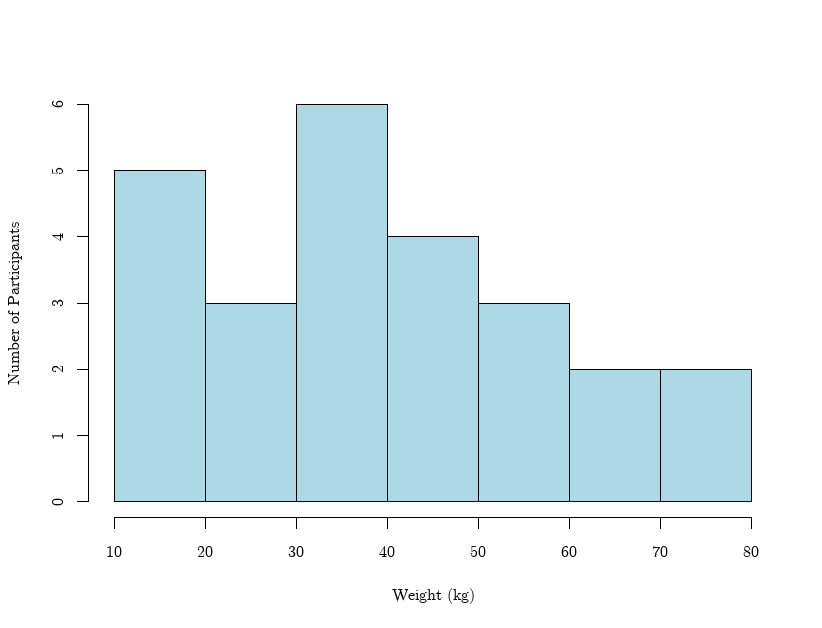
\includegraphics[width=0.9\textwidth]{graph2/HistWeight.png}
			  \caption{Histogram of Subjects' Weights}
			  \label{fig:histogram}
			\end{minipage}\hfill
			\begin{minipage}{0.46\textwidth}
			  \centering
			  \tiny
			  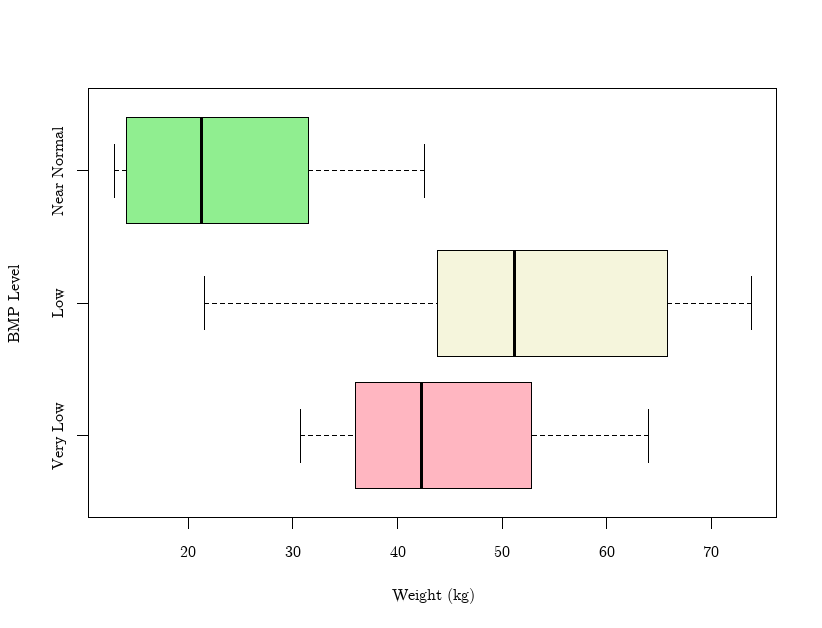
\includegraphics[width=0.9\textwidth]{graph2/BoxWeight.png}
			  \caption{Distribution of Subject Weights Aggregated by BMP Level}
			  \label{fig:boxplots}
			\end{minipage}
		\end{figure}
		
		\begin{figure}[h!]
			\centering
			\tiny
			\begin{minipage}{0.46\textwidth}
			  \centering
			  \tiny
			  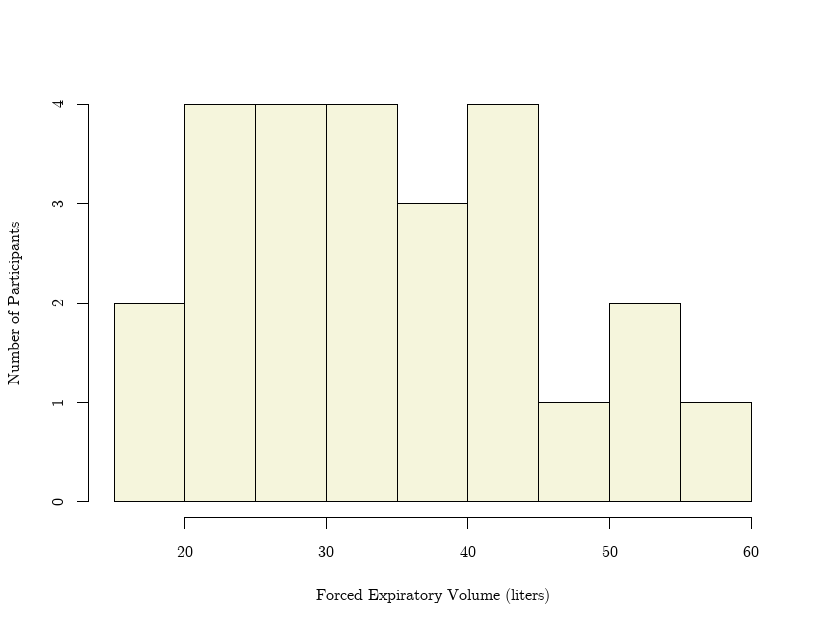
\includegraphics[width=0.9\textwidth]{graph2/HistFEV.png}
			  \caption{Histogram of Subjects' FEV1}
			  \label{fig:histogram}
			\end{minipage}\hfill
			\begin{minipage}{0.46\textwidth}
			  \centering
			  \tiny
			  \includegraphics[width=0.9\textwidth]{graph2/bmpbar.png}
			  \caption{Distribution of Subjects across BMP Levels}
			  \label{fig:boxplots}
			\end{minipage}
		\end{figure}

		We found evidence to support a correlation between weight and forced expiratory volume in one second $(p = 0.0196, \rho = 0.4637)$. This finding was backed up by the sensitivity analysis ($p = 0.0141, \tau = 0.3518)$. Additionally, within this study, we did not find evidence to suggest that age was a significant cofounder in determining the FEV1 of a subject.

		\begin{table}[h]
			\centering
			\footnotesize
			\renewcommand{\arraystretch}{1.2}
			\caption{Correlation Found Between Weight \& FEV1, but not Age and FEV1}
			\begin{tabular}{lcccc}
				\toprule
				& \multicolumn{2}{c}{Spearman’s $\rho$} & \multicolumn{2}{c}{Kendall’s $\tau$} \\
				\cmidrule(lr){2-3} \cmidrule(lr){4-5}
				& $\rho$ & p-value & $\tau$ & p-value \\
				\midrule
				Weight \& FEV1 & $0.4637$ & 0.0196 & $0.3518$ & 0.0141 \\
				Age \& FEV1 & $0.2974$ & 0.1487 & $0.2173$ & 0.1386 \\
				\bottomrule
			\end{tabular}
		\end{table}

		\newpage

		\begin{figure}[h!]
			\centering
			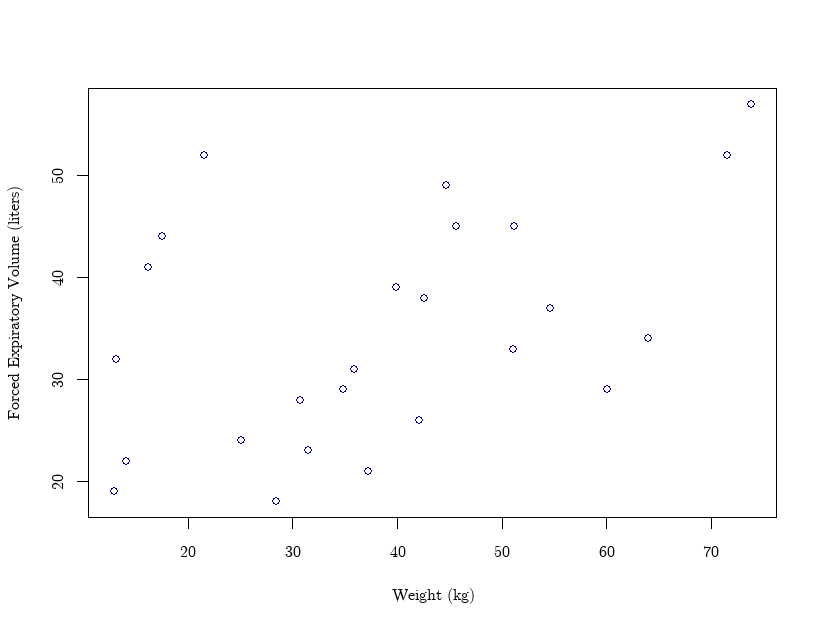
\includegraphics[width=0.6\textwidth]{graph2/ScatterWeightFEV.png}
			\caption{Correlation Found Between Weight and Forced Expiratory Volume}
			\label{fig:histogram}
		\end{figure}


		We found evidence to support a correlation between weight and forced expiratory volume in one second $(p = 0.0196, \rho = 0.4637)$. This finding was supported by the sensitivity analysis ($p = 0.0141, \tau = 0.3518)$. Additionally, within this study, we did not find evidence to suggest that age was a significant cofounder in determining the FEV1 of a subject. 
		
		
		We also found evidence to suggest that there was a difference in FEV1 levels at different levels of BMP within the subjects $(p = 0.0424, H = 6.324, df = 2)$, supported by the separation of the BMP groups in figure 8. Post-hoc tests with a Bonferroni adjustment reveal that there was a difference in FEV1 values between participants who had a very low BMP and a near-normal BMP, as shown in Table 5, but an insignificant difference between the other groups.


		\begin{table}[h!]
			\centering
			\caption{Post-Hoc Mann-Whitney U Test Show Difference in FEV Between Very Low \& Near-Normal Body Mass Proportion}
			\footnotesize
			\begin{tabular}{l c c c}
			\toprule
			\textbf{Comparison} & \textbf{W Statistic} & \textbf{p-value} & \textbf{Significant at $\alpha^* = 0.0167$} \\
			\midrule
			Very Low - Low      & 29                   & 0.3599          & No  \\
			Normal - Low        & 41.5                 & 0.1314          & No  \\
			Very Low \& Normal  & 10                   & 0.01667         & Yes \\
			\bottomrule
			\end{tabular}
		\end{table}

		\subsection*{Discussion}
		Overall, we have found statistically significant evidence of positive correlation between weight and FEV1, but not BMP. Kerem and colleagues (2013) also found that BMI was a contributor to FEV1 in cystic fibrosis patients, as well as chronic Pseudomonas aeruginosa infection, pancreatic status, and CF-related diabetes. Their statistically significant analyses showed that patients with a poor BMI had, on average, 21.6\% lower FEV1 percentage predicted than patients with a normal BMI. However, they also found that FEV1 was overall negatively associated with age, over their sample of 6 to >45 year olds. Future analyses should be mindful of the demography of their samples, as well as changing patterns in lung function across the lifespan as technologies and average life expectancy of CF patients increase (Balasa \& Chaudary, 2020), and adjust their statistical approaches and assumptions accordingly. Other studies of young children show an analogous relationship between BMI and FEV1 (Sanders et al., 2015). In any case, future studies should expand sample sizes where possible in order to lessen variability and enhance power.
		
		\newpage
		\subsection*{Appendix}
		\begin{itemize}
			\item Balasa, G., \& Chaudary, N. (2020). The Lung Life of a Cystic Fibrosis Patient: A Patient and Physician Perspective. Pulmonary Therapy, 6, 159-167. 
			https://doi.org/10.1007/s41030-020-00130-9
			\item Kerem, E., Viviani, L., Zolin, A., MacNeill, S., Hatziagorou, E., Ellemunter, H., Drevinek, P., Gulmans, V., Krivec, U., \& Olesen, H. (2013). Factors associated with FEV1 decline in cystic fibrosis: analysis of the ECFS Patient Registry. European Respiratory Journal, 43(1), 125-133. 
			https://doi.org/10.1183/09031936.00166412
			\item Sanders, D. B., Emerson, J., Ren, C. L., Schechter, M. S., Gibson, R. L., Morgan, W., \& Rosenfeld, M. (2015). Early Childhood Risk Factors for Decreased FEV1 at Age Six to Seven Years in Young Children with Cystic Fibrosis. Annals of the American Thoracic Society, 12(8), 1170-1176. 
			https://doi.org/10.1513/AnnalsATS.201504-198OC
		\end{itemize}

		\subsection*{R Code}

		\begin{lstlisting}[language=R, basicstyle=\tiny]
			# formatting stuff (add latex font)
			library(showtext)
			library(DescTools)
			library(Rfit)
			font_add(family = 'ComputerModern', regular = 'cmunrm.ttf') # for consistent formatting in LaTex
			showtext_auto()
			par(family = 'ComputerModern')
			# end formatting stuff
			
			cf <- read.table('cf.txt', header = TRUE)
			
			# for separating dataframes and parsing through to get summaries
			vLow = subset(cf, bmp == 'Very Low')
			low = subset(cf, bmp == 'Low')
			norm = subset(cf, bmp == 'Near Normal')
			bodyMasses = list(all = cf, veryLow = vLow, someLow = low, nearNorm = norm)
			
			# loop for summary stats
			for (group_name in names(bodyMasses)) {
			
			  # mean age
			  # mean wt
			  # median wt
			  # mean fev1
			  # median fev1
			  group_data = bodyMasses[[group_name]]
			  wt_sd <- sd(group_data$weight)
			  fev_sd = sd(group_data$fev1)
			  n <- length(group_data$age)
			  wt_margin = qt(0.975, df = n - 1) * (wt_sd / sqrt(n))
			  fev_margin = qt(0.975, df = n - 1) * (fev_sd / sqrt(n))
			
			  print(paste('Group:', group_name, '( N =', n, ')')) # for future reference: paste() used to concatenate strings
			  print(paste('  Mean Age:', round(mean(group_data$age), 3))) # prints mean age
			  print(paste('  Mean Weight:', round(mean(group_data$weight), 3)))
			  print(paste('  Weight 95% CI:', round(wt_margin, 3)))
			  print(paste('  Median Weight:', round(median(group_data$weight), 3)))
			
			  print('')
			  print(paste('  Mean FEV:', round(mean(group_data$fev1), 3)))
			  print(paste('  FEV 95% CI:', round(fev_margin, 3)))
			  print(paste('  Median FEV:', round(median(group_data$fev1), 3)))
			  print('')
			}
			
			for (group_name in names(exposures)) {
			  group_data = exposures[[group_name]]
			
			  vital_sd <- sd(group_data$vital.capacity)
			  n <- length(group_data$vital.capacity)
			
			  margin = qt(0.975, df = n - 1) * (vital_sd / sqrt(n))  # margin for 95% CI
			
			  # print results
			  print(paste('Group:', group_name, '( N =', n, ')')) # for future reference: paste() used to concatenate strings
			  print(paste('  Mean Age:', round(mean(group_data$age), 3))) # prints mean age
			  print(paste('  Mean Vital Capacity:', round(mean(group_data$vital.capacity), 3),
						  '| SD:', round(vital_sd, 3)))
			  print(paste('  95% CI MoE:', round(margin, 3)))
			  print(paste('  Median VC:', median(group_data$vital.capacity)))
			  print(paste('  MAD:', mad(group_data$vital.capacity)))
			  print('')
			}
			
			hist(cf$weight, col = 'lightblue',
				 xlab = 'Weight (kg)', ylab = 'Number of Participants',
				 main = '')
			
			hist(cf$fev1, col = 'beige',
				 xlab = 'Forced Expiratory Volume (liters)', ylab = 'Number of Participants',
				 main = '')
			
			boxplot(weight ~ bmp, data = cf, 
					main = '',
					xlab = 'Weight (kg)', 
					ylab = 'BMP Level', 
					col = c('lightpink', 'beige', 'lightgreen'), horizontal = T,
					names = c('Very Low', 'Low', 'Near Normal'))
			
			bmpfreq <- table(cf$bmp)

			barplot(bmpfreq,
			        main = '',
			        xlab = 'BMP Level', 
			        ylab = 'Frequency', 
			        col = c('lightpink', 'beige', 'lightgreen'), horizontal = T,
			        names = c('Very Low', 'Low', 'Near Normal'))
			
			# Spearmans
			with(cf, cor.test(fev1, weight, method = 'spearman'))
			with(cf, cor.test(fev1, weight, method = 'kendall'))
			plot(fev1 ~ weight, data = cf, col = 'darkblue',
				 xlab = 'Weight (kg)', ylab = 'Forced Expiratory Volume (liters)')
			
			# Age
			with(cf, cor.test(fev1, age, method = 'spearman'))
			with(cf, cor.test(fev1, age, method = 'kendall'))
			
			# Post-hocs
			kruskal.test(fev1 ~ bmp, data = cf)
			wilcox.test(vLow$fev1, low$fev1)
			wilcox.test(norm$fev1, low$fev1)
			wilcox.test(vLow$fev1, norm$fev1)
			
			vLow = subset(cf, bmp == 'Very Low')
			low = subset(cf, bmp == 'Low')
			norm = subset(cf, bmp == 'Near Normal')
			\end{lstlisting}
			
			






		


		
\end{document}














